\begin{table*}[tb]
\small
\centering
\caption{Five Original Datasets}
\begin{tabular}{|c|l|r|r|r|r|} \hline
Dataset	& Description & Recs & Dom. & Sensitive & Non-Sens.\\
& & & Size & items & items  \\ \hline \hline
BMS-POS &Point-of-sale data from &515597 & 1657&1183355 &  2183665\\
(POS)	& a large electronics retailer   &	&	&	& \\ \hline
BMS-WebView &Click-stream data from &77512 & 3340& 137605 & 220673  \\
(WV) & e-commerce web site  & &  & & \\ \hline
Retail &  Retail market basket data   & 88162&16470 &340462 & 568114  \\ \hline
Syn & Synthetic data with max & 493193 &5000 &828435 & 1242917 \\
 & record length = 50   & & & & \\ \hline
\end{tabular}
\label{tab:datasets}
\end{table*}

\section{Experimental Results}
\label{sec:eval}

We conducted a series of experiments on
4 main datasets in Table \ref{tab:datasets}. BMS-POS and BMS-WebView are
introduced in \cite{Zheng:2001:RWP:502512.502572} and are commonly used for
data mining. Retail is the retail market basket data \cite{brijs99:retailData}. Syn is the synthetic data in which each item is generated with 
equal probability and the max record length is 50.
%Figure \ref{fig:datasets}  shows the record length distribution
%of the four datasets.
% Since there is no distinction of sensitive data from non-sensitive data,
We randomly designate 40\% of the item types in each dataset as
sensitive items and the rest as non-sensitive.
To evaluation the performance of rule mining,
we produce four additional datasets by truncating all records in the
original datasets to 5 items only, and denote
such datasets as ``cutoff = 5''.

We compare our algorithm with the
global suppression algorithm (named Global) and generalization algorithm 
(named TDControl) of
Cao {\em et al.} \cite{Cao:2010:rho}.\footnote{The source code of these
algorithms was directly obtained from Cao.} 
%since these systems are most
%related to our work in terms of privacy model. In the rest of the section,
%by {\em Global} and {\em TDControl}, we mean these two algorithms.
Our algorithm has two variants, {\em Dist} and {\em Mine}, which optimize
for data distribution and rule mining, respectively.
%We also compare the performance of the above algorithms with a simple
%baseline algorithm denoted as {\em Random} which
%randomly picks one unsafe \qid and one item type in this \qid to suppress.
%In order to evaluate the ability to retain useful association rules and
%to avoid spurious rules in these competing algorithms, we need the ground
%truth, which are all the association rules inferrable from the datasets with
%sufficient confidence and support.
%However, original datasets are too large to infer all association rules.
Experiments that failed to complete in 2 hours is marked
as ``N/A'' or an empty place in the bar charts.
 %However, both TDControl and global
 %suppression are unavailable in large datasets, thus we cannot make %comparisons in Syn-1 and Syn-2 and Retail where $\rho=0.3$
 %with them.
%reported by Cao \etal \cite{Cao:2010:rho}
%against the same data sets.
%Cao {\em et al.} were very supportive of our work and gave us their code directly.
We run all the experiments on Linux 2.6.34)
with an Intel 16-core 2.4GHz CPU and 8GB RAM. 
%Experiment programs are written in C++ and compiled using GCC version 4.5.0.

In what follows, we first present results in data utility, then the
performance of the algorithms, and then the effects of
changing various parameters in our algorithm. 
Finally, we compare with a permutation method which utilizes
a similar privacy model but with different optimization goals. 
Unless otherwise noted, we use the following default parameters: 
$b_{max} = 10^6$ , $t_{max}=500$. 

\subsection{Data Utility}\label{sec:eval:datautility}
We compare the algorithms in terms of information loss, data distribution,
and association rule mining.

\begin{figure}[tb]
\centering
\subfigure[ $\rho=0.3$]{\label{fig:loss-a}
\hspace{-4mm}
\begin{minipage}[c]{0.4\textwidth}
  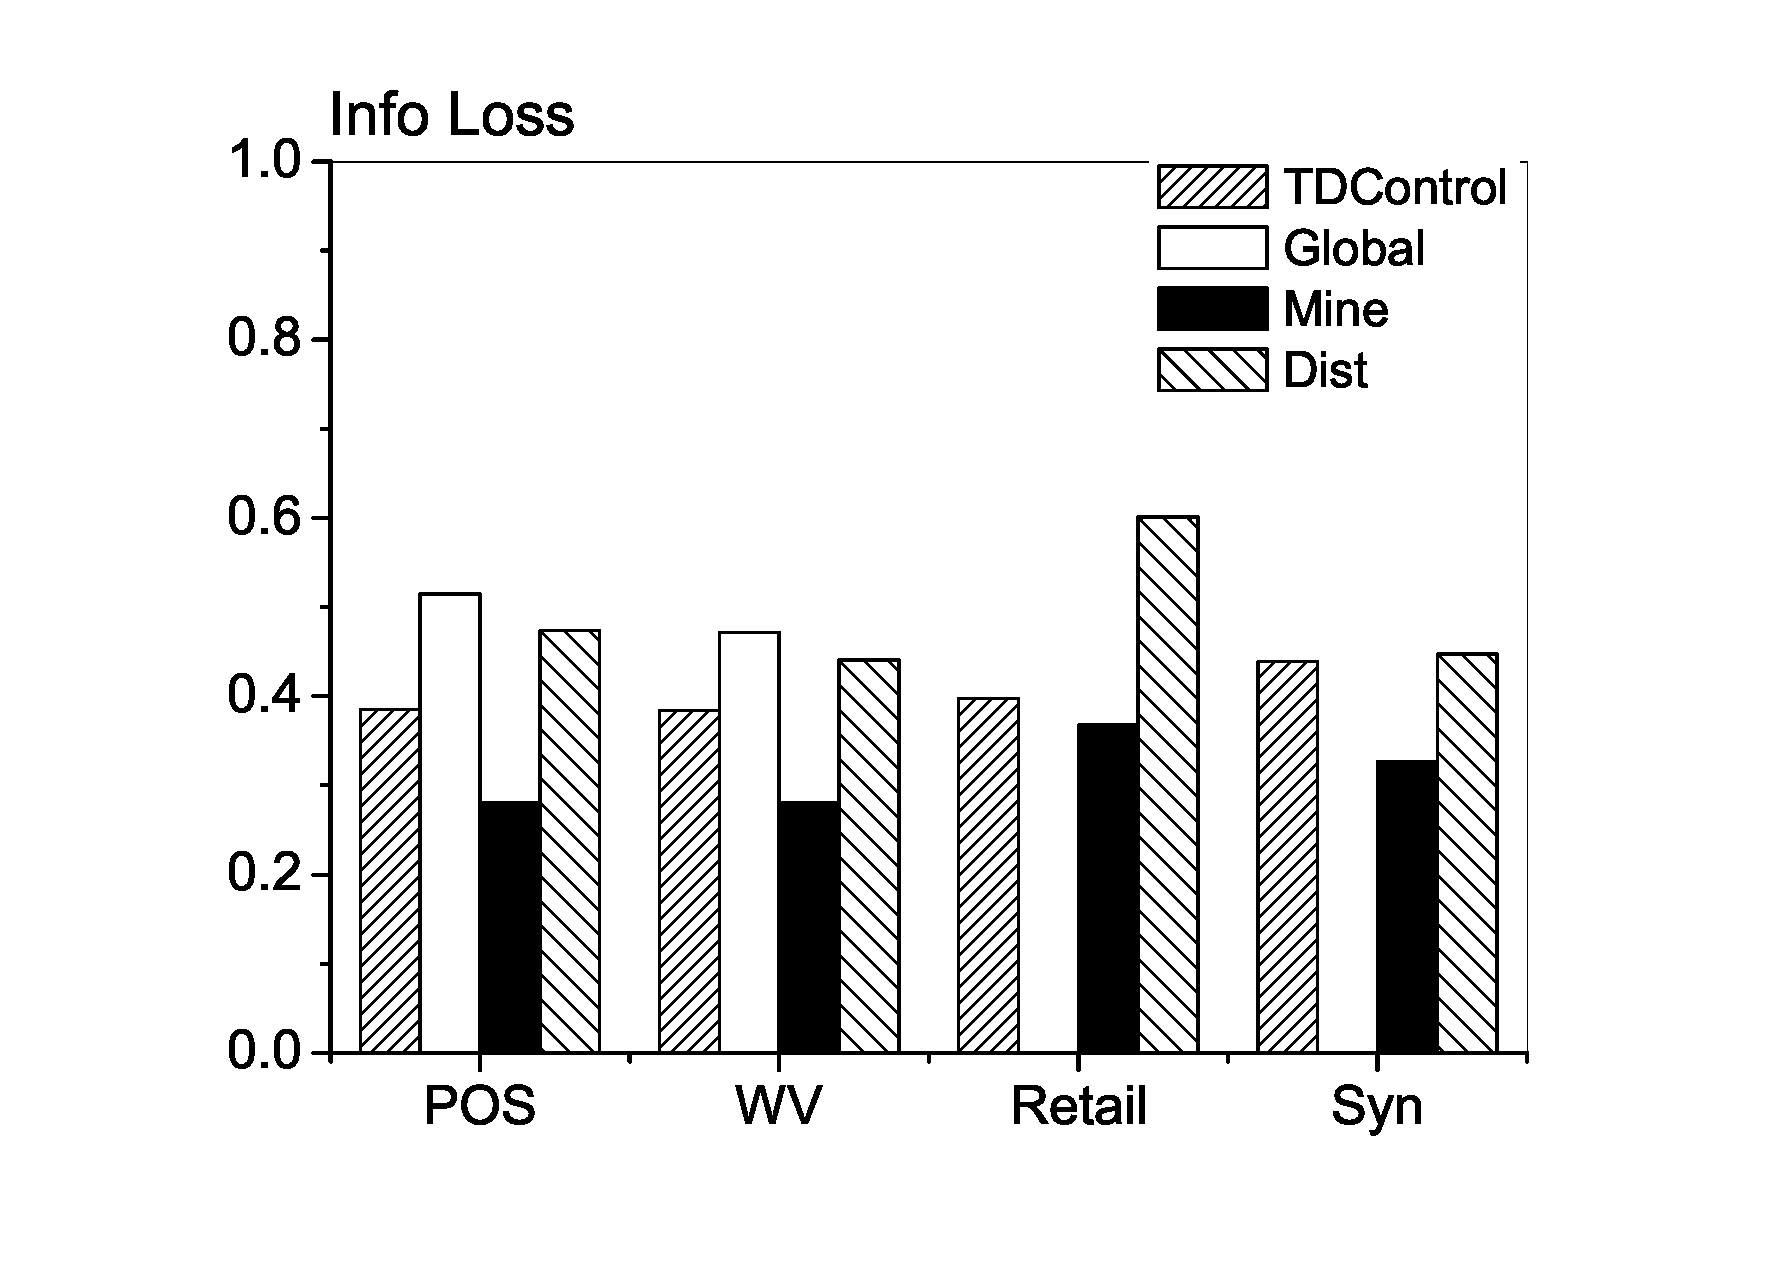
\includegraphics[width=5cm]{loss3.eps}
\end{minipage}%
}
\subfigure[ $\rho=0.7$]{\label{fig:loss-b}
\begin{minipage}[c]{0.4\textwidth}
  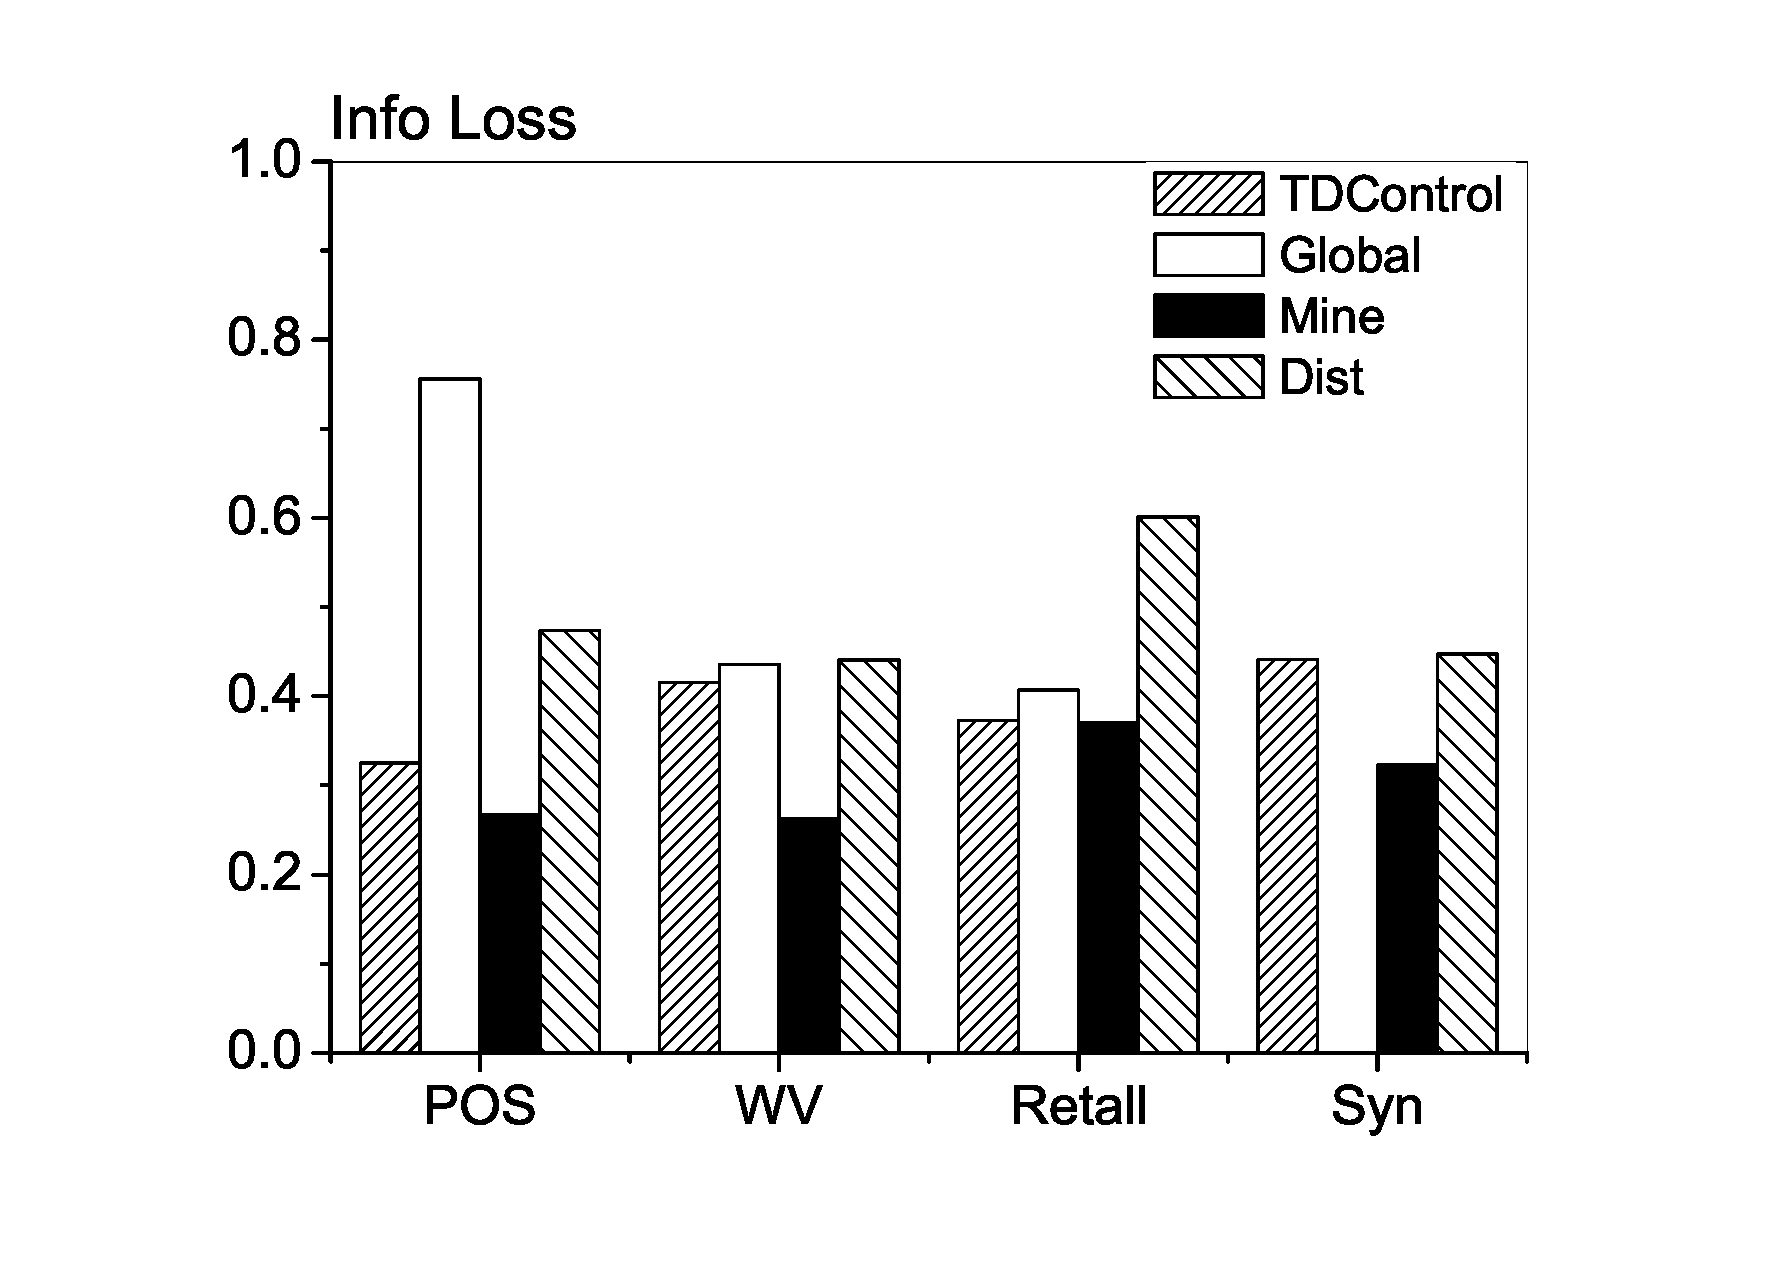
\includegraphics[width=5cm]{loss7.eps}
\end{minipage}%
}
\caption{Comparisons in Information Loss}\label{fig:loss}
\end{figure}

Figure \ref{fig:loss}
shows that $Mine$ is uniformly better among the other four techniques.
It suppresses only about 26\% items in POS and WV and about 35\% items in
Retail, while the other four techniques incur on average 10\% more losses
than  $Mine$ and up to 75\% losses in the worst case. We notice that $Dist$
performs worse than  $Global$ even though it tries to minimize the
information loss at each iteration.
The reason is that it also tries to retain the data
distribution. 
%We will see how this heuristic works in retaining the data
%distribution in Section \ref{sec:eval:datadistribution}.
Further, we argue that for applications that require data statistics,
the distribution, that is, summary information, is more useful than the
details, hence losing some detailed information is acceptable.
Note that Global and TDControl failed to complete in some datasets,
because these methods don't scale very well.
%This confirms that our alogrithm causes less information losses than peers.
%which suggests that our algorithm scales better on bigger data than the
%existing approaches.
%indicating that our algorithm has a
%strong flexibility in $\rho$.

%\subsubsection{Data Distribution}\label{sec:eval:datadistribution}

\begin{figure}[tb]
\centering
\subfigure[ $\rho=0.3$]{
\hspace{-4mm}
\begin{minipage}[c]{0.4\textwidth}
\centering
  \includegraphics[width=5cm]{relative3.eps}
\end{minipage}%
}
\subfigure[ $\rho=0.7$]{
\begin{minipage}[c]{0.4\textwidth}
\centering
  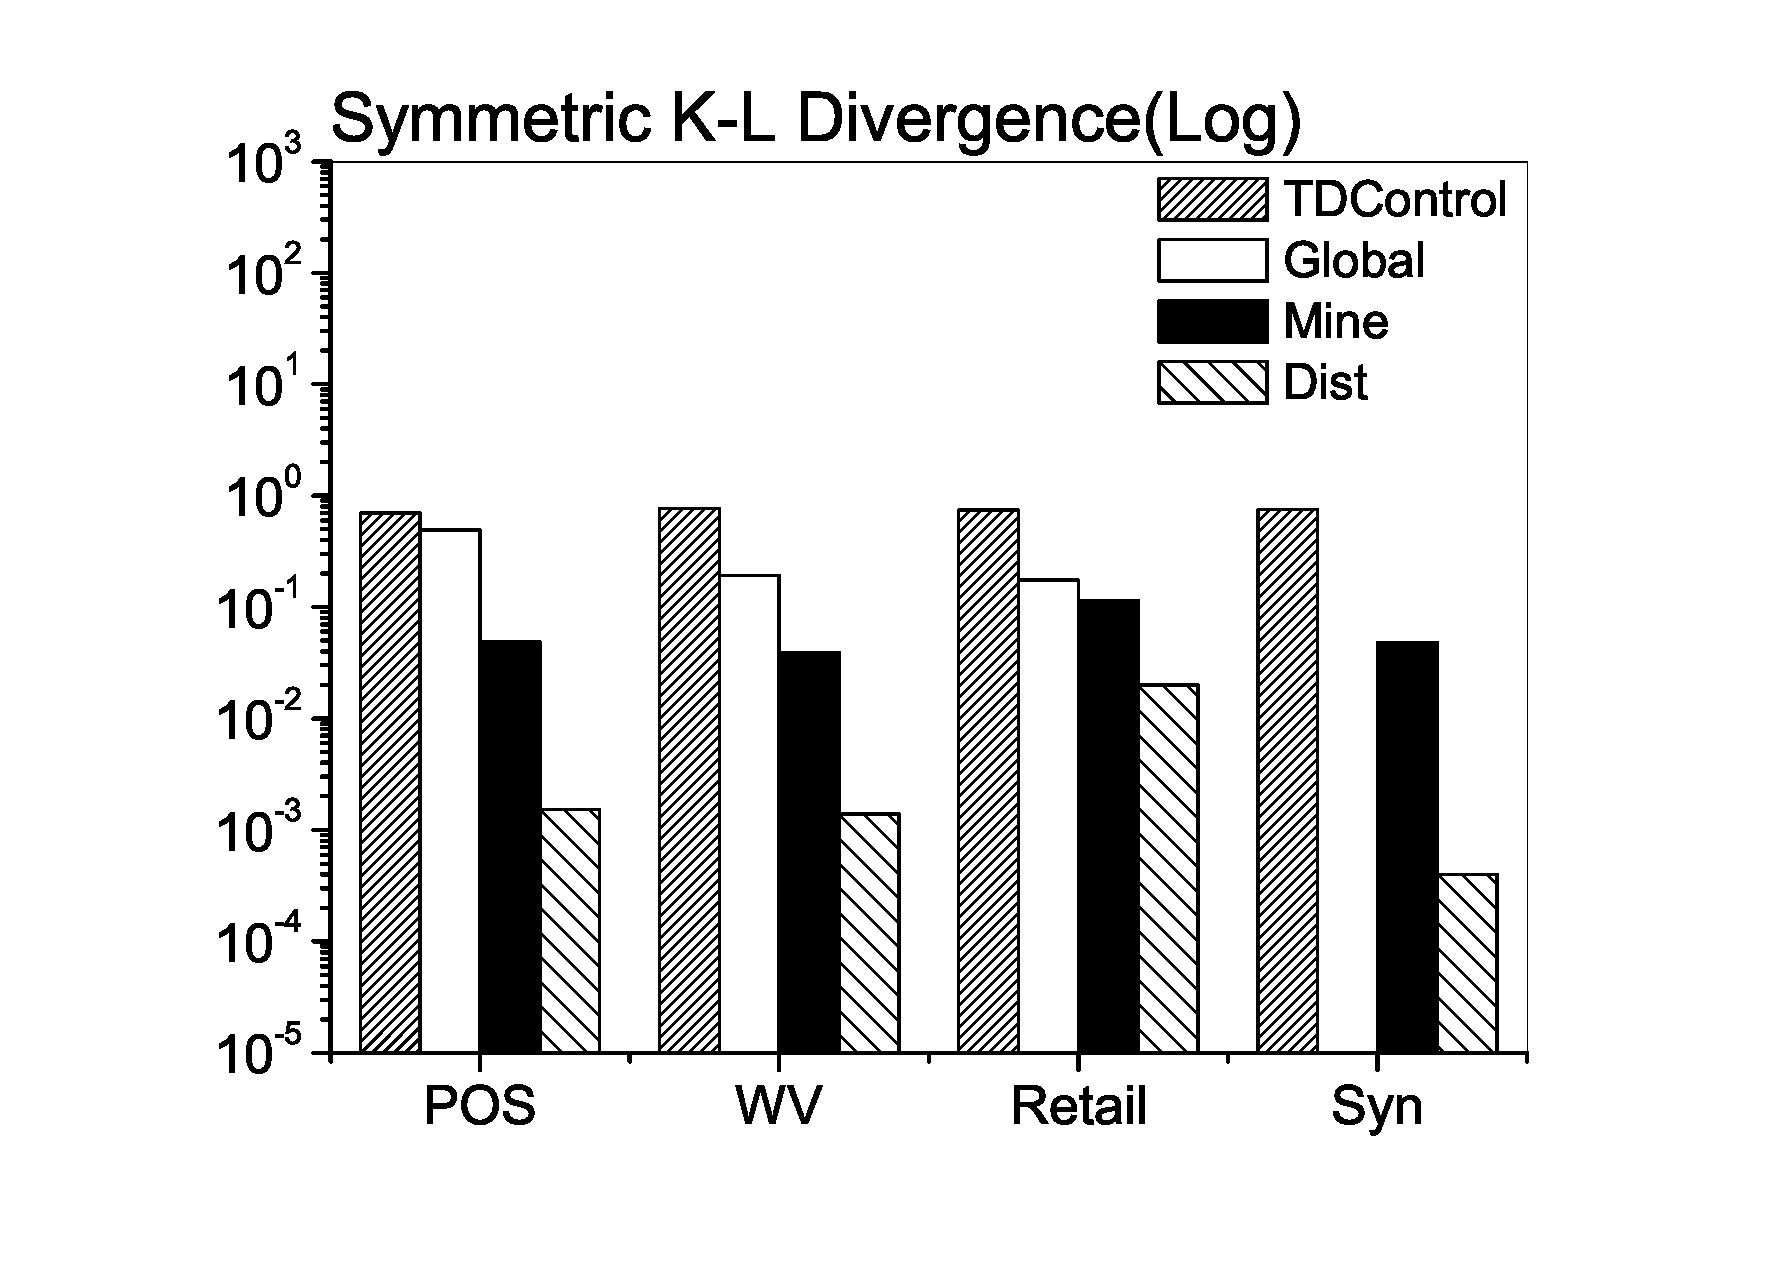
\includegraphics[width=5cm]{relative7.eps}
\end{minipage}%
}
\caption{Comparisons in Symmetric K-L Divergence}
\label{fig:entropy}
\end{figure}

To determine the similarity between the item frequency distribution
of original data and that of the anonymized data,
we use the Kullback-Leibler
divergence (also called relative entropy) as our standard.
To prevent zero denominators, we modified \eqnref{eq:kl-dis}
to a symmetric form \cite{Fisher:2008:DSF} defined as
\[\mathcal{S}(H_1||H_2)=\frac{1}{2}KL( H_1||H_1 \oplus H_2)+\frac{1}{2} KL( H_2||H_1 \oplus H_2)\]
where  $H_1 \oplus H_2$ represents the union of distributions $H_1$ and $H_2$.
Figure \ref{fig:entropy} shows that $Dist$ outperforms the peers
 as its output has the highest resemblance
to the original datasets.
On the contrary, TDControl is the worst performer
since generalization algorithm creates a lot of new items while
suppressing too many item types globally.
Since the symmetric relative entropy of $Dist$ is very small, y-axis is
in logrithmic scale to improve visibility. Therefore, the actual difference
in K-L divergence is two or three orders of magnitude.
% We only show the results of $Dist$ heuristics here since $Dist$ is supposed to
% preserve the data distribution.  However, the other two partial suppression
% strategies also outperform global and TDControl in this respect, only to
% a lesser extent. 

The most common criticism of partial suppression is that it
changes the support of good rules in the data and introduces spurious
rules in rule mining. In this experiment, we test the algorithms on
data sets with the max record length=5 (cutoff=5),
and check the rules mined from the anonymized data
with support equals to 0.05\% \footnote{We choose this support level just to
reflect a practical scenario.} and confidence equals to 70\% and 30\%.
%Mining rules from the original datasets with many
%long records is prohibitive due to large memory requirements.
Figure \ref{fig:rulemining} gives the results.
Both TDControl and Global perform badly in this category, with
negligible number of original rules remaining after anonymization.
Conversely, all of the partial
suppression algorithms manage to retain most of the rules and the Jaccard Similarity reaches 80\% in some datasets which shows
our heuristic works very well. 
Specifically, $Mine$ performs the best among partial algorithms. 
The rules generated from TDControl are all in general form which is
totally different from the original one. To enable comparison,
we specialize the more general rules from the result of TDControl
into rules of original level of abstraction in the generalization hierarchy.
For example, we can specialize a rule \{dairy product $\rightarrow$ grains\}
into:
\rm{milk} $\rightarrow$ \rm{wheat}, 
\rm{milk} $\rightarrow$ \rm{rice}, 
\rm{yogurt} $\rightarrow$ \rm{wheat}, etc. 
%\rm{yogurt} $\rightarrow$ \rm{rice}\\
Take WV as an example, there are 4 rules left in the result of TDControl when
the $\rho$ is 0.7 and the number becomes 28673 after specialization, which makes
the results almost invisible.

\begin{figure}[tb]
\centering
\subfigure[ $\rho=0.3$]{
\hspace{-4mm}
\begin{minipage}[c]{0.4\textwidth}
\centering
   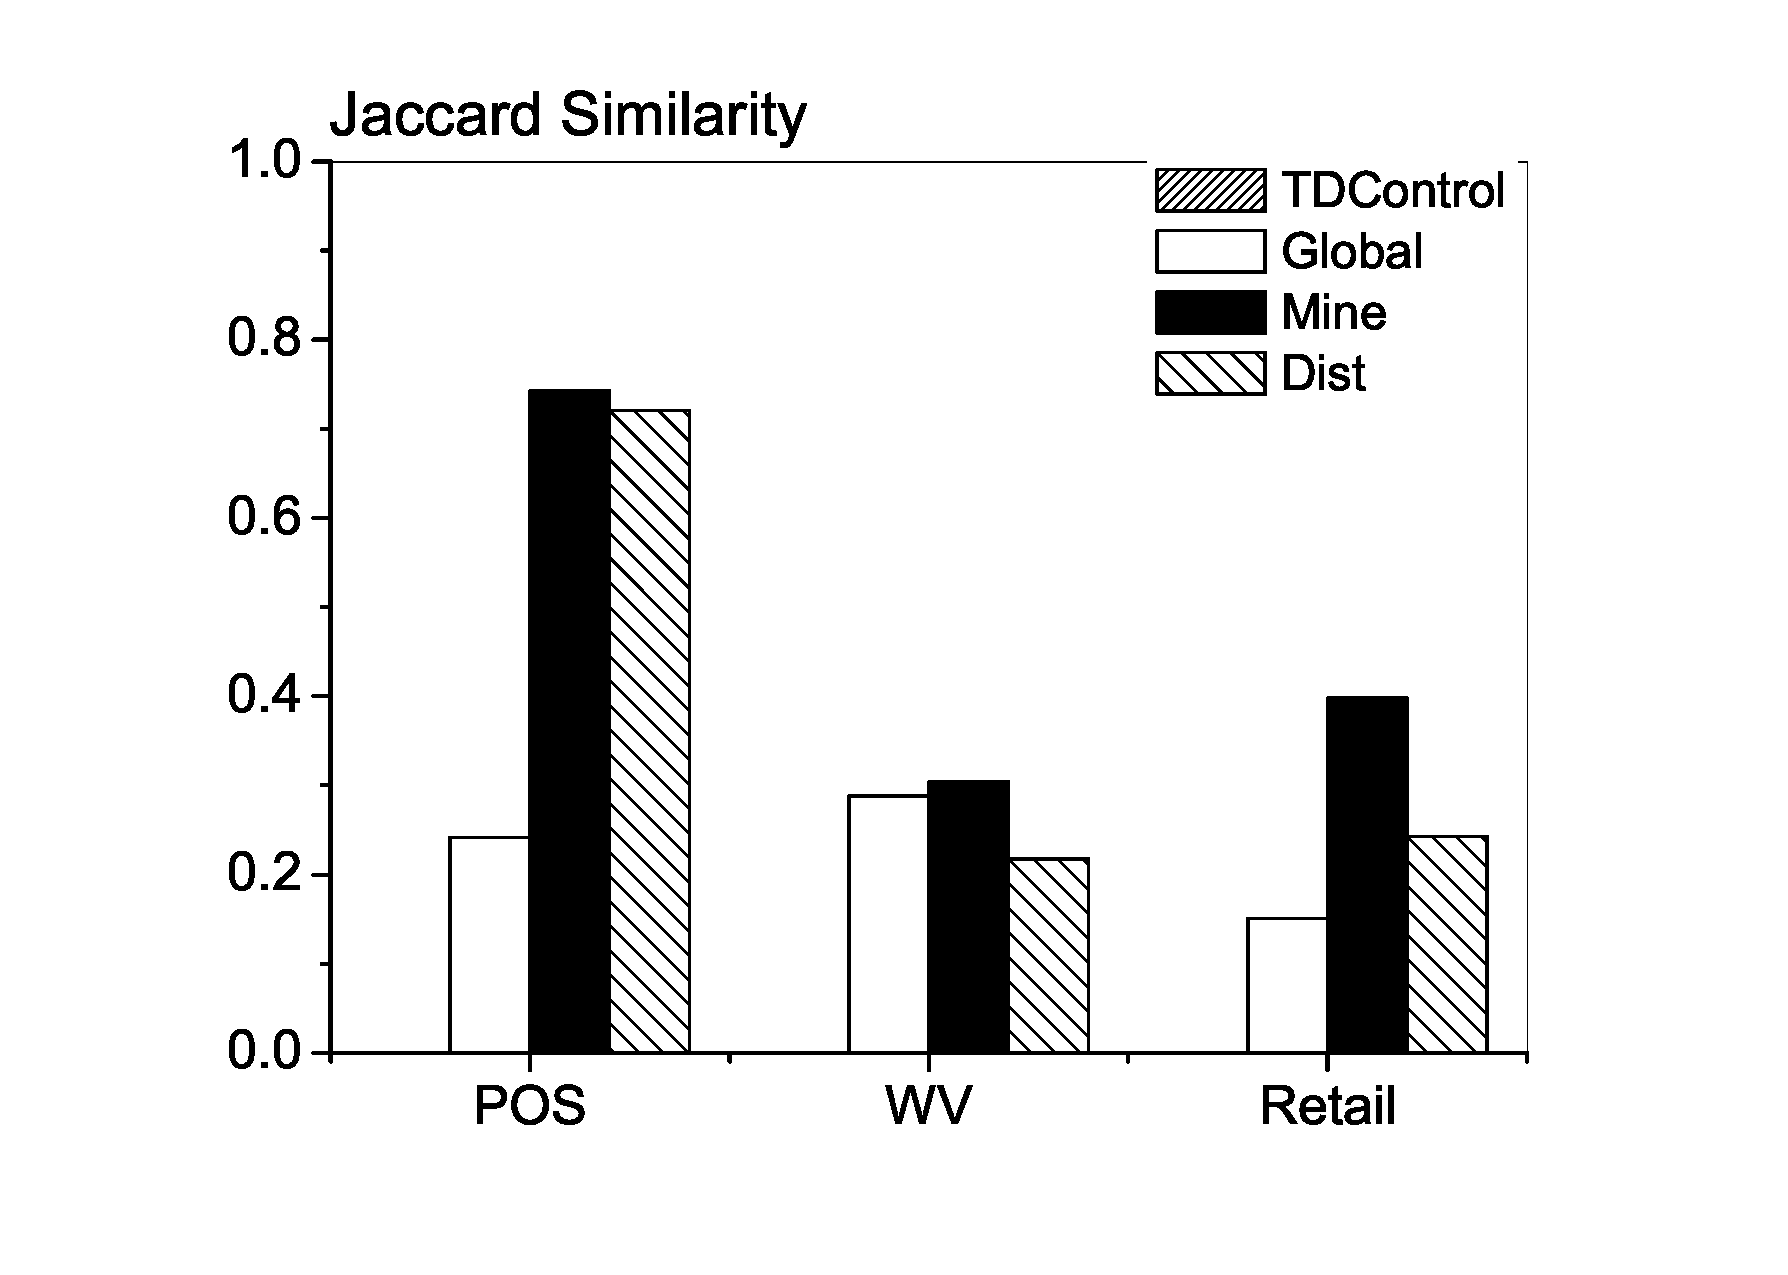
\includegraphics[width=5cm]{js3.eps}\\
\end{minipage}%
}
\subfigure[ $\rho=0.7$]{
\begin{minipage}[c]{0.4\textwidth}
\centering
  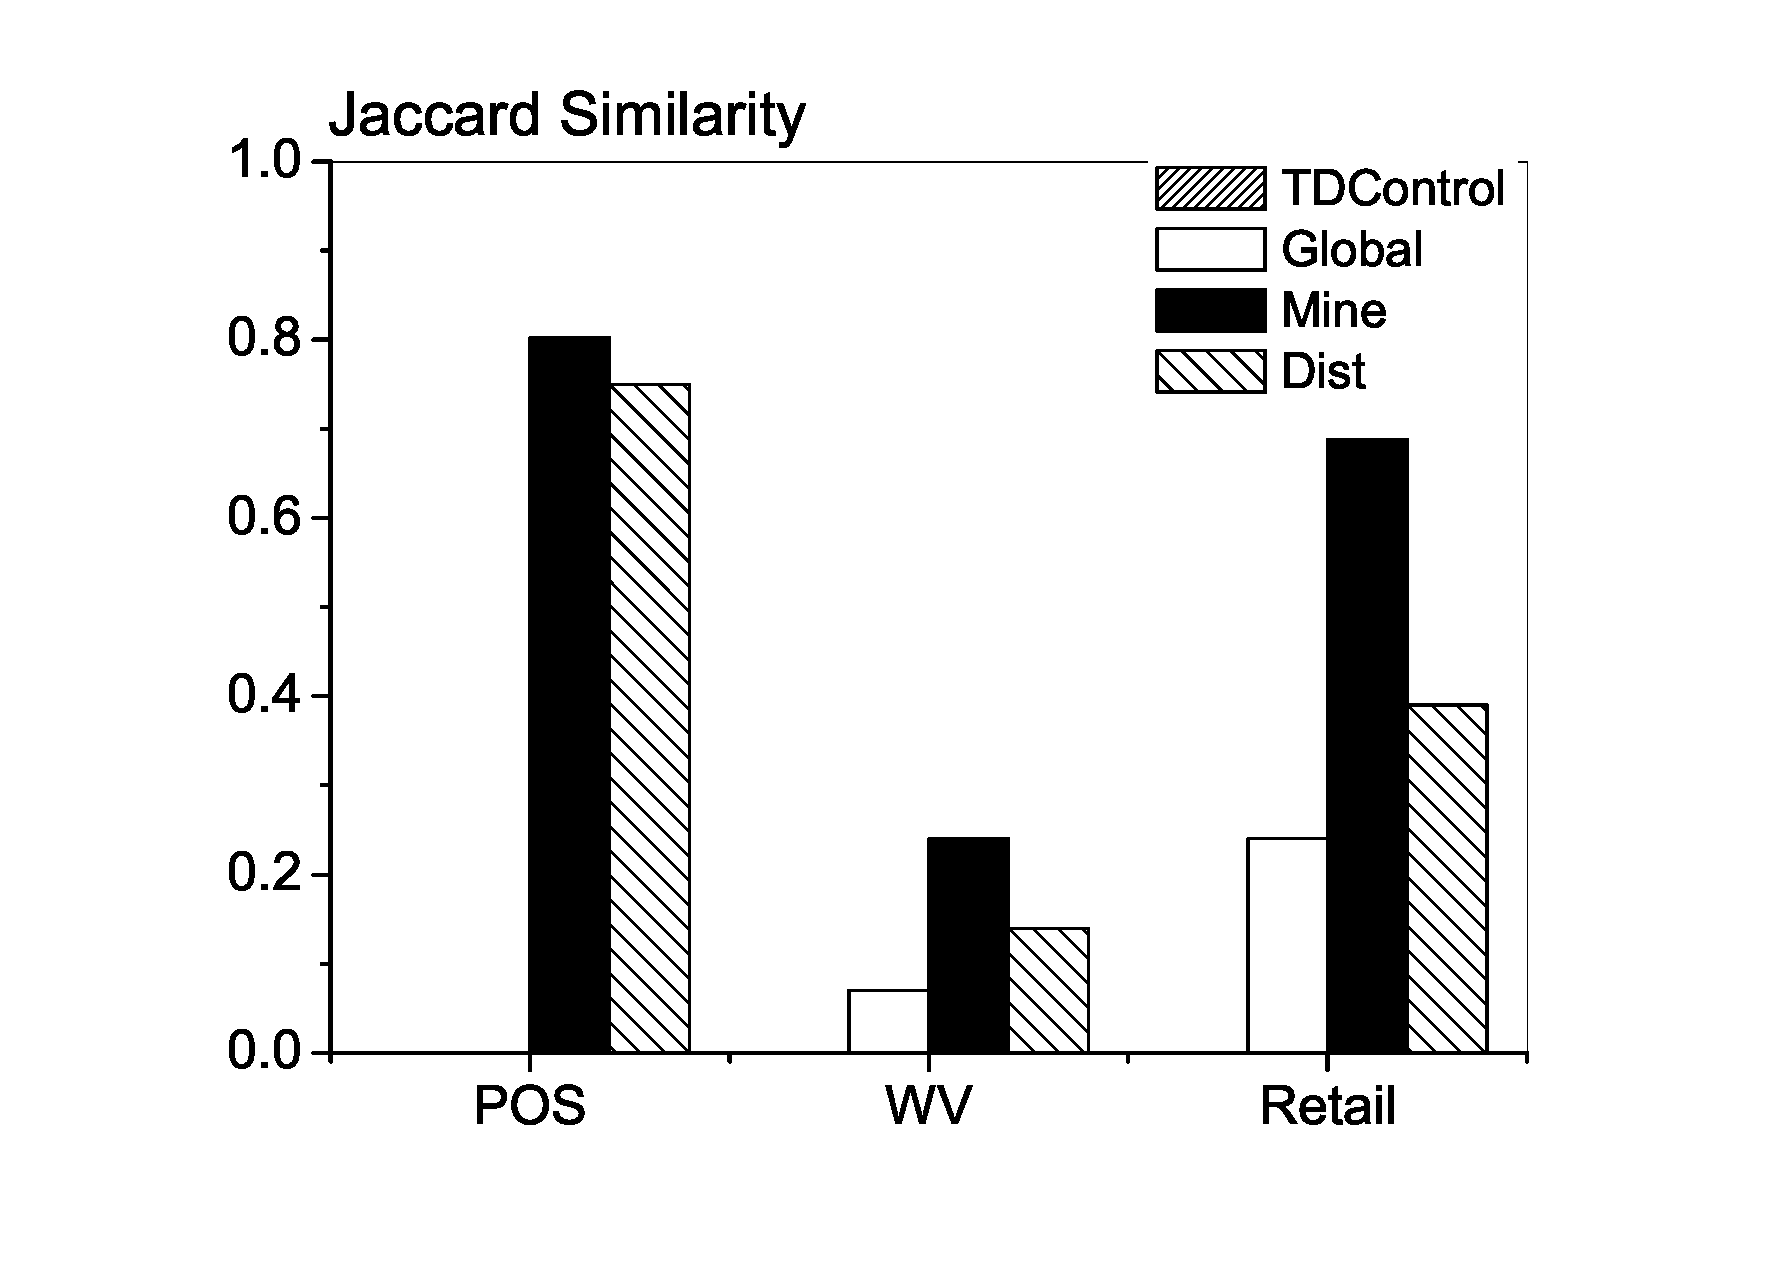
\includegraphics[width=5cm]{js7.eps}
\end{minipage}%
}
 \caption{Association Rules Mining with Support $0.05 \%$}
 \label{fig:rulemining}
\end{figure}

\subsection{Performance}\label{sec:eval:performance}
Next we evaluate the time performance and scalability of
our algorithms.

%\subsubsection{Time Performance}\label{sec:eval:time}
\begin{table}[bh]
\caption{Comparison in Time Performance ($\rho=0.7$, $t_{max}=300$)}
\centering
\begin{tabular}{|l|r|r|r|r|r|}
  \hline
  % after \\: \hline or \cline{col1-col2} \cline{col3-col4} ...
  Algorithm & POS & WV & Retail  &Syn \\  \hline \hline
  TDControl & \bf{183} & \bf{30 }& \bf{156} &   476  \\  \hline
  Global & 1027 & 81 & 646 &   N/A  \\  \hline
%  \PartialR & 6582 & 305 & 1497 & 323&761 \\\hline
 % $Random$ & 814 & 188 & \bf{151} & \bf{105} \\\hline
  $Dist$ & 395 & 151 & 171 &\bf{130}\\ \hline
  $Mine$ & 1554 & 478& 256 & 132\\ \hline
  \end{tabular}
\label{tab:timeresult}
\end{table}

%Since data anonymization often takes place in offline mode,
%time performance is often not critical.
%Nonetheless, time matters if we want our algorithm to
%scale to large datasets.
%But reasonable time performance is still important for a data user.
From Table \ref{tab:timeresult}, TDControl is the clear winner
for two of the four datasets. $Mine$ does not perform well in BMS-POS.
The reason is that $Mine$ incurs the least information loss among all the
competiting methods. This means most of the original data remains
unsuppressed. Given the large scale of BMS-POS, checking whether the
dataset is safe in each iteration is therefore more time consuming than
other methods or in other datasets.
Results for Global are not available for Syn because
it runs out of memory.

%\subsubsection{Scalability}\label{sec:eval:scale}
Next experiment illustrates the scalability of our algorithm
w.r.t. data size. We choose $Retail$ as our target dataset here
%since the number of \qids increases dramatically with
%the increase of the records length
because $Retail$ has the maximum average record length of 10.6.
We run partial algorithms on 1/5, 2/5 through 5/5 of $Retail$ respectively.
Figure \ref{fig:scale} shows 
the time cost of our algorithm increases reasonably with the 
input data size with or without DnC.
%On Retail with DnC, data is partitioned into
%two pieces at 2/5 data, four pieces at 3/5 and 4/5 data, and then
%eight pieces for the whole data.
Furthermore, increased level of partitioning causes the algorithm to witness
superlinear speedup in Figure \ref{fig:scale:a}. In particular, the dataset is
automatically divided into 4, 8, 16 and 32 parts at 1/5, 2/5, 3/5 and
the whole of the data, respectively.
\begin{figure}[tb]
\centering
\subfigure[With DnC]{\label{fig:scale:a}
\hspace{-4mm}
\begin{minipage}[c]{0.4
\textwidth}
\centering
  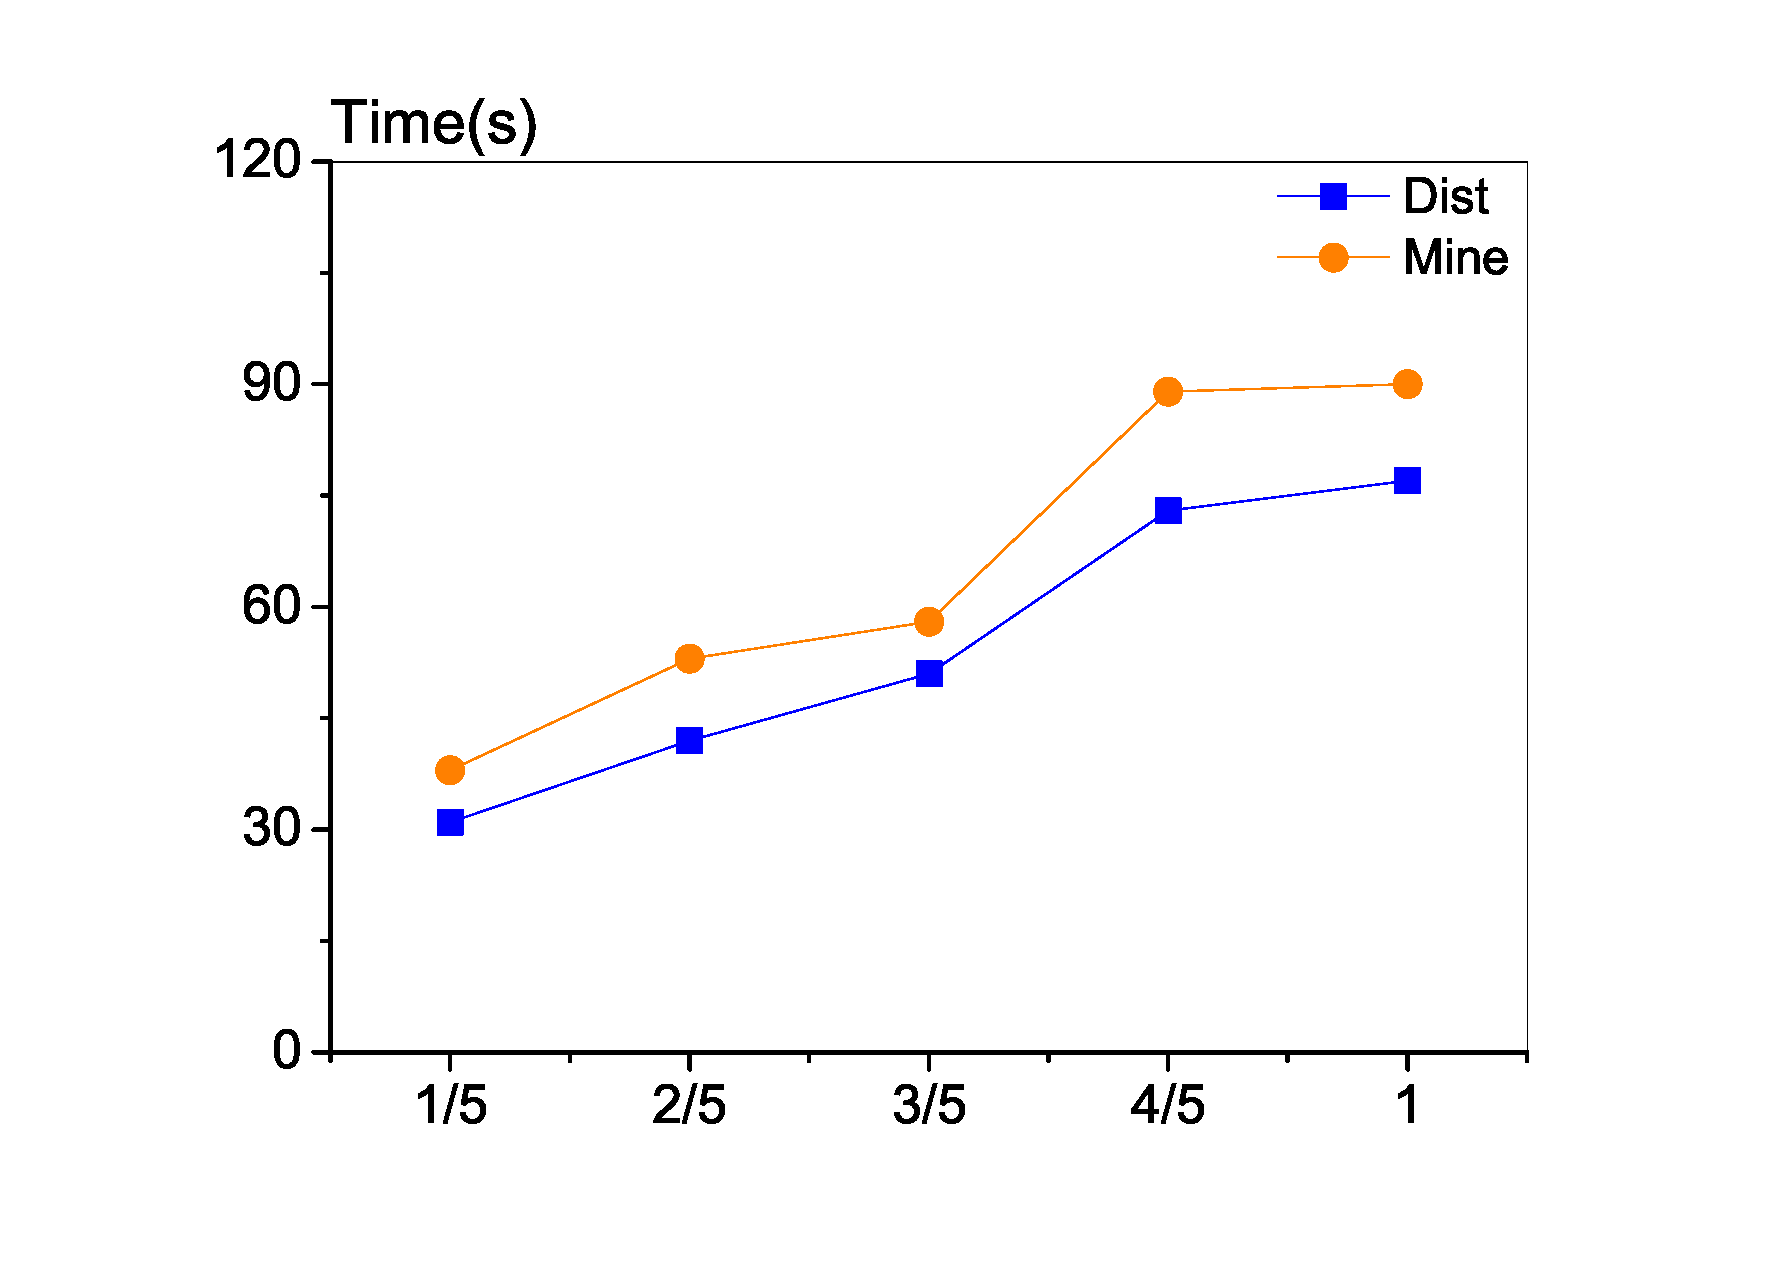
\includegraphics[width=5cm]{scaletime.eps}
\end{minipage}%
}
\subfigure[Without DnC]{\label{fig:scale:b}
\begin{minipage}[c]{0.4\textwidth}
\centering
  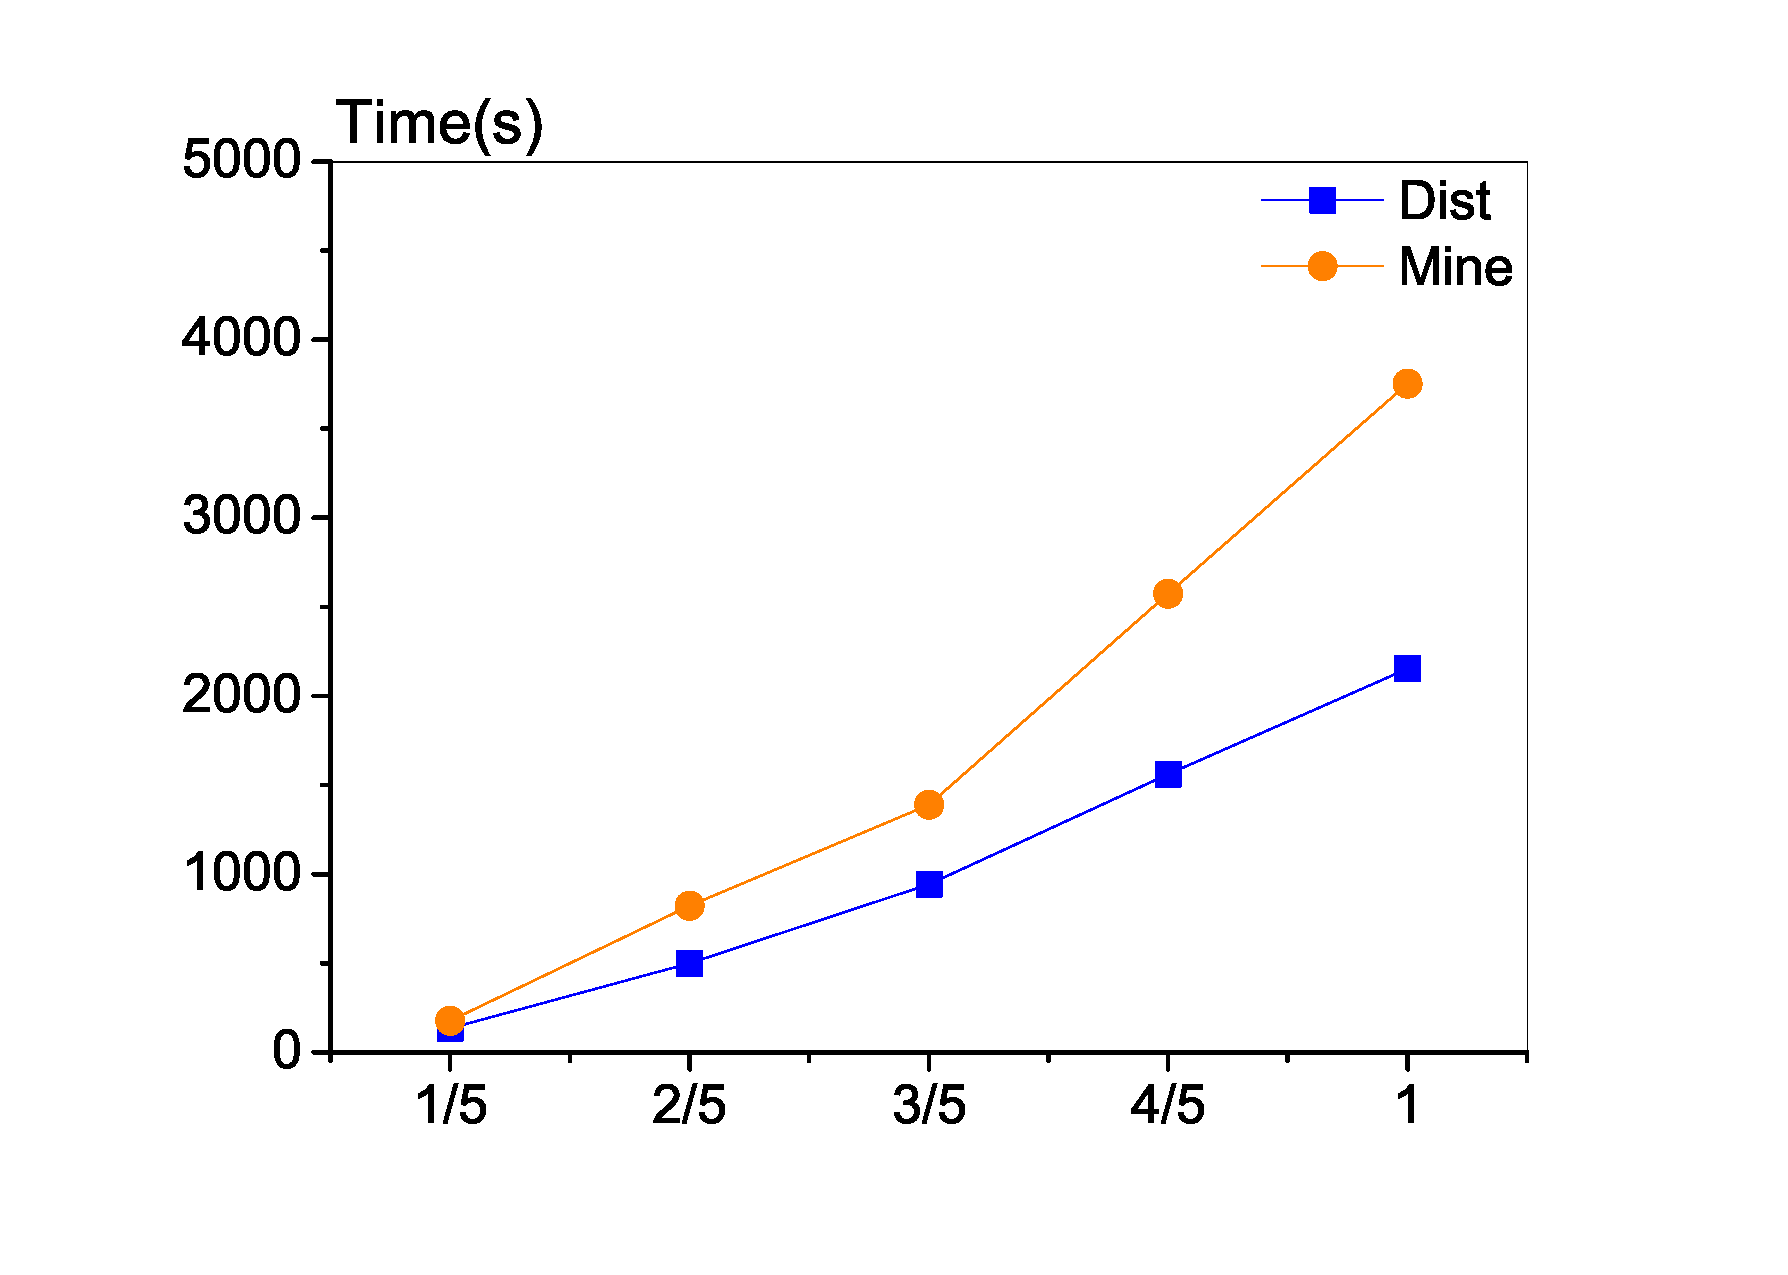
\includegraphics[width=5cm]{scaletimeno.eps}
\end{minipage}%
}
\caption{Scale-up with Input Data ($\rho=0.7$)}\label{fig:scale}
\end{figure}

\subsection{Effects of Parameters on Performance}\label{sec:eval:effect}
In this section, 
%we analyze the trade-offs in three variants of our basic algorithm, and 
we study the effects of $t_{max}$, $b_{max}$ on the
quality of solution (in terms of information loss) and time performance.
%parameters for optimization defined in our algorithm help to ameliorate the time performance by the largest extent but remain the quality of the suppressed datasets.
%We have 4 different parameters including partial suppression policies

%\subsubsection{Variation of $t_{max}$}\label{sec:eval:timebound}
We choose $Retail$ as the target dataset again since $Retail$
is the most time-consuming dataset that can terminate within
acceptable time without DnC strategy.
The value of $t_{max}$ determines the size of a partition in DnC. 
%Smaller $t_{max}$ can give rise to more partitions. 
Here, we evaluate how partitioning helps with time performance and
its possible effects on suppression quality.
Figure \ref{fig:timebound-a} shows the relationship between partitions
and information loss. The lines of  $Dist$ is flat, indicating that
increasing $t_{max}$ doesn't cost us the quality of the solution. $Mine$
shows a slight descending tendency at first and then tends to be flat.
We argue that a reasonable $t_{max}$ will not cause our result quality to
deteriorate.
On the other hand, Figure \ref{fig:timebound-b} shows that
time cost increases dramatically  with the increase of  $t_{max}$.
The reason is that partitioning decreases the cost of enumerating \qids which
is the most time-consuming part in our algorithm. Moreover, parallel
processing is also a major reason for the acceleration.

%timebound
\begin{figure}[tb]
\centering
\subfigure[Information Loss]{
\label{fig:timebound-a}
\hspace{-4mm}
\begin{minipage}[c]{0.4\textwidth}
\centering
  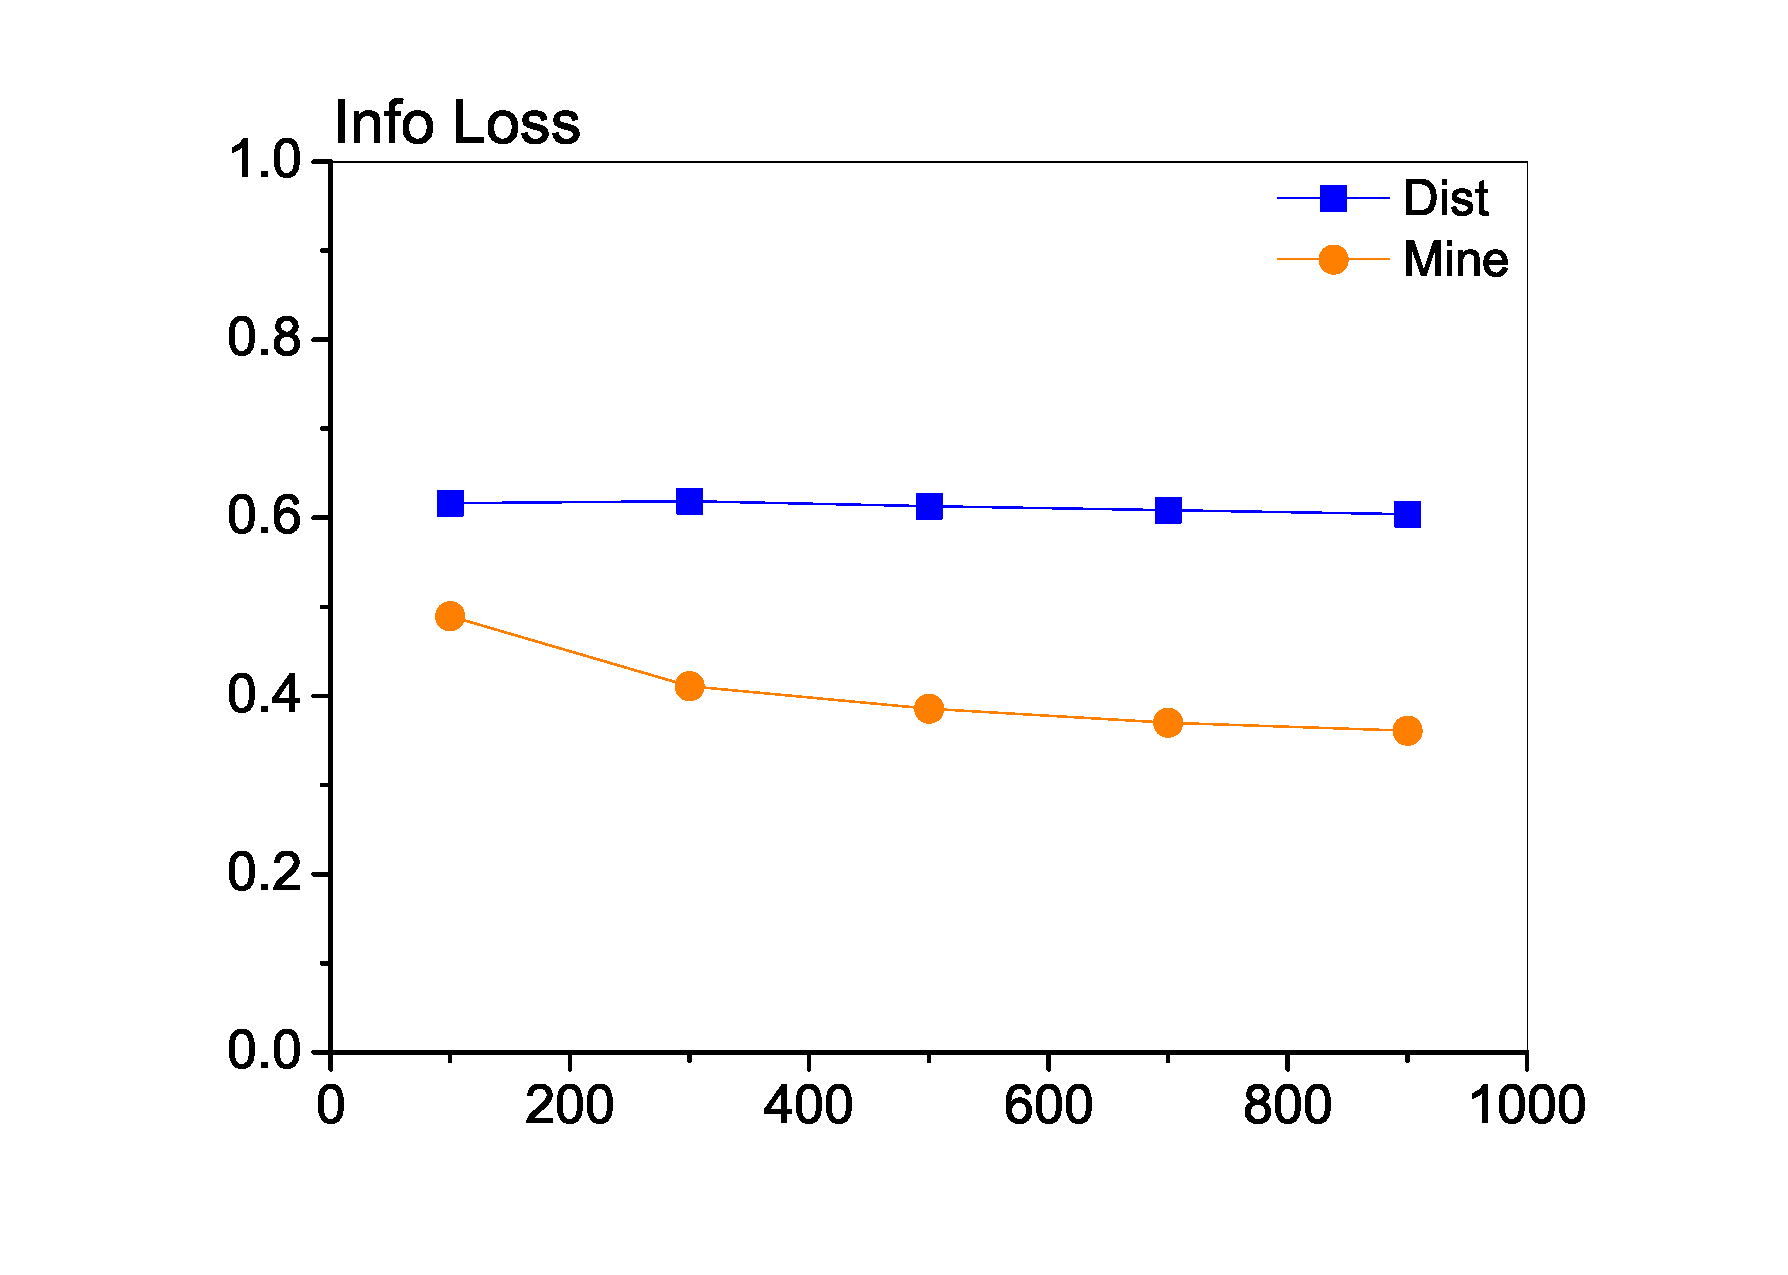
\includegraphics[width=5cm]{timebond_avg.eps}
\end{minipage}%
}
\subfigure[Time Performance]{
\label{fig:timebound-b}
\begin{minipage}[c]{0.4\textwidth}
\centering
  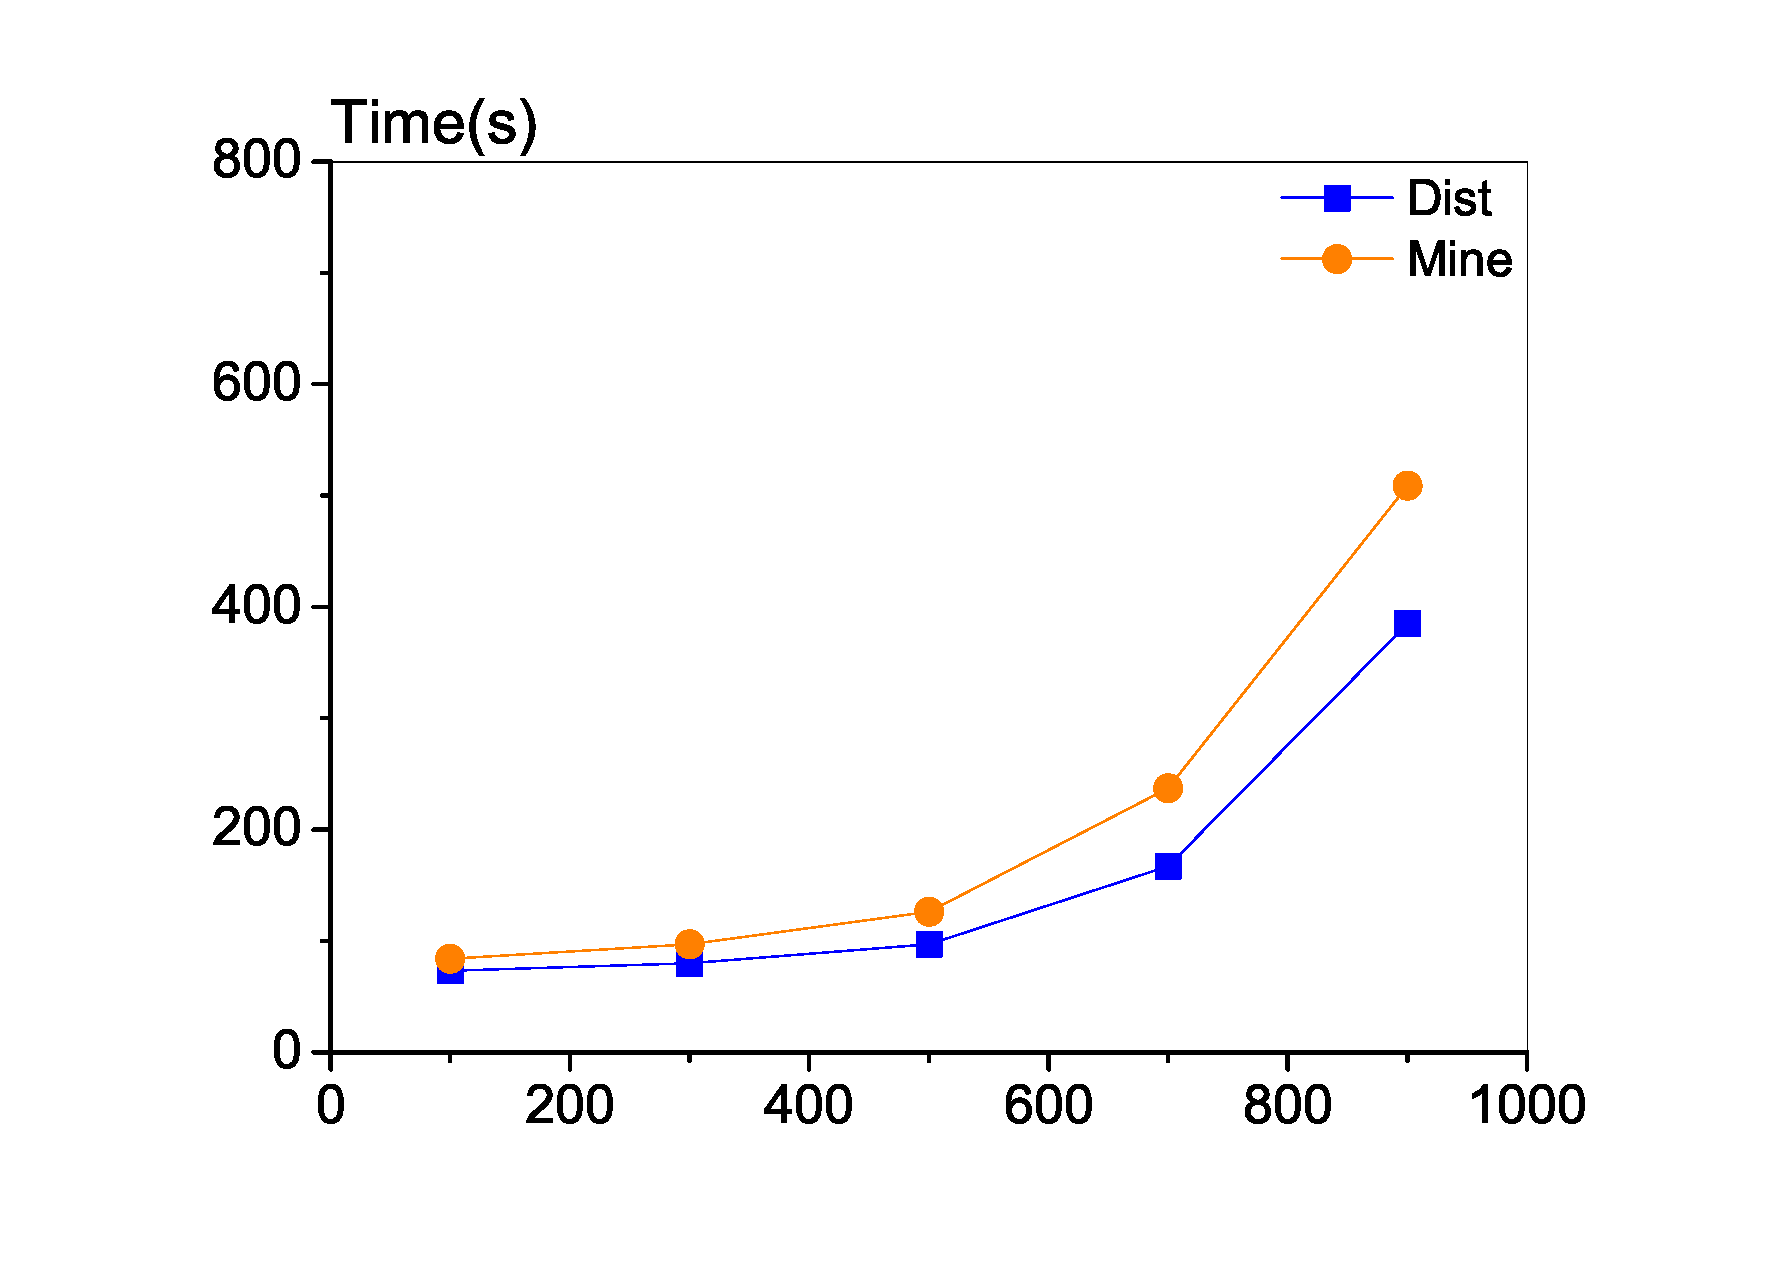
\includegraphics[width=5cm]{timebond.eps}
\end{minipage}%
}
\caption{Variation of $t_{max}$ ($\rho = 0.7$)}\label{fig:timebound}
\end{figure}

\begin{figure}[tb]
\centering
\subfigure[Information Loss]{
\hspace{-4mm}
\begin{minipage}[c]{0.4
\textwidth}
\centering
  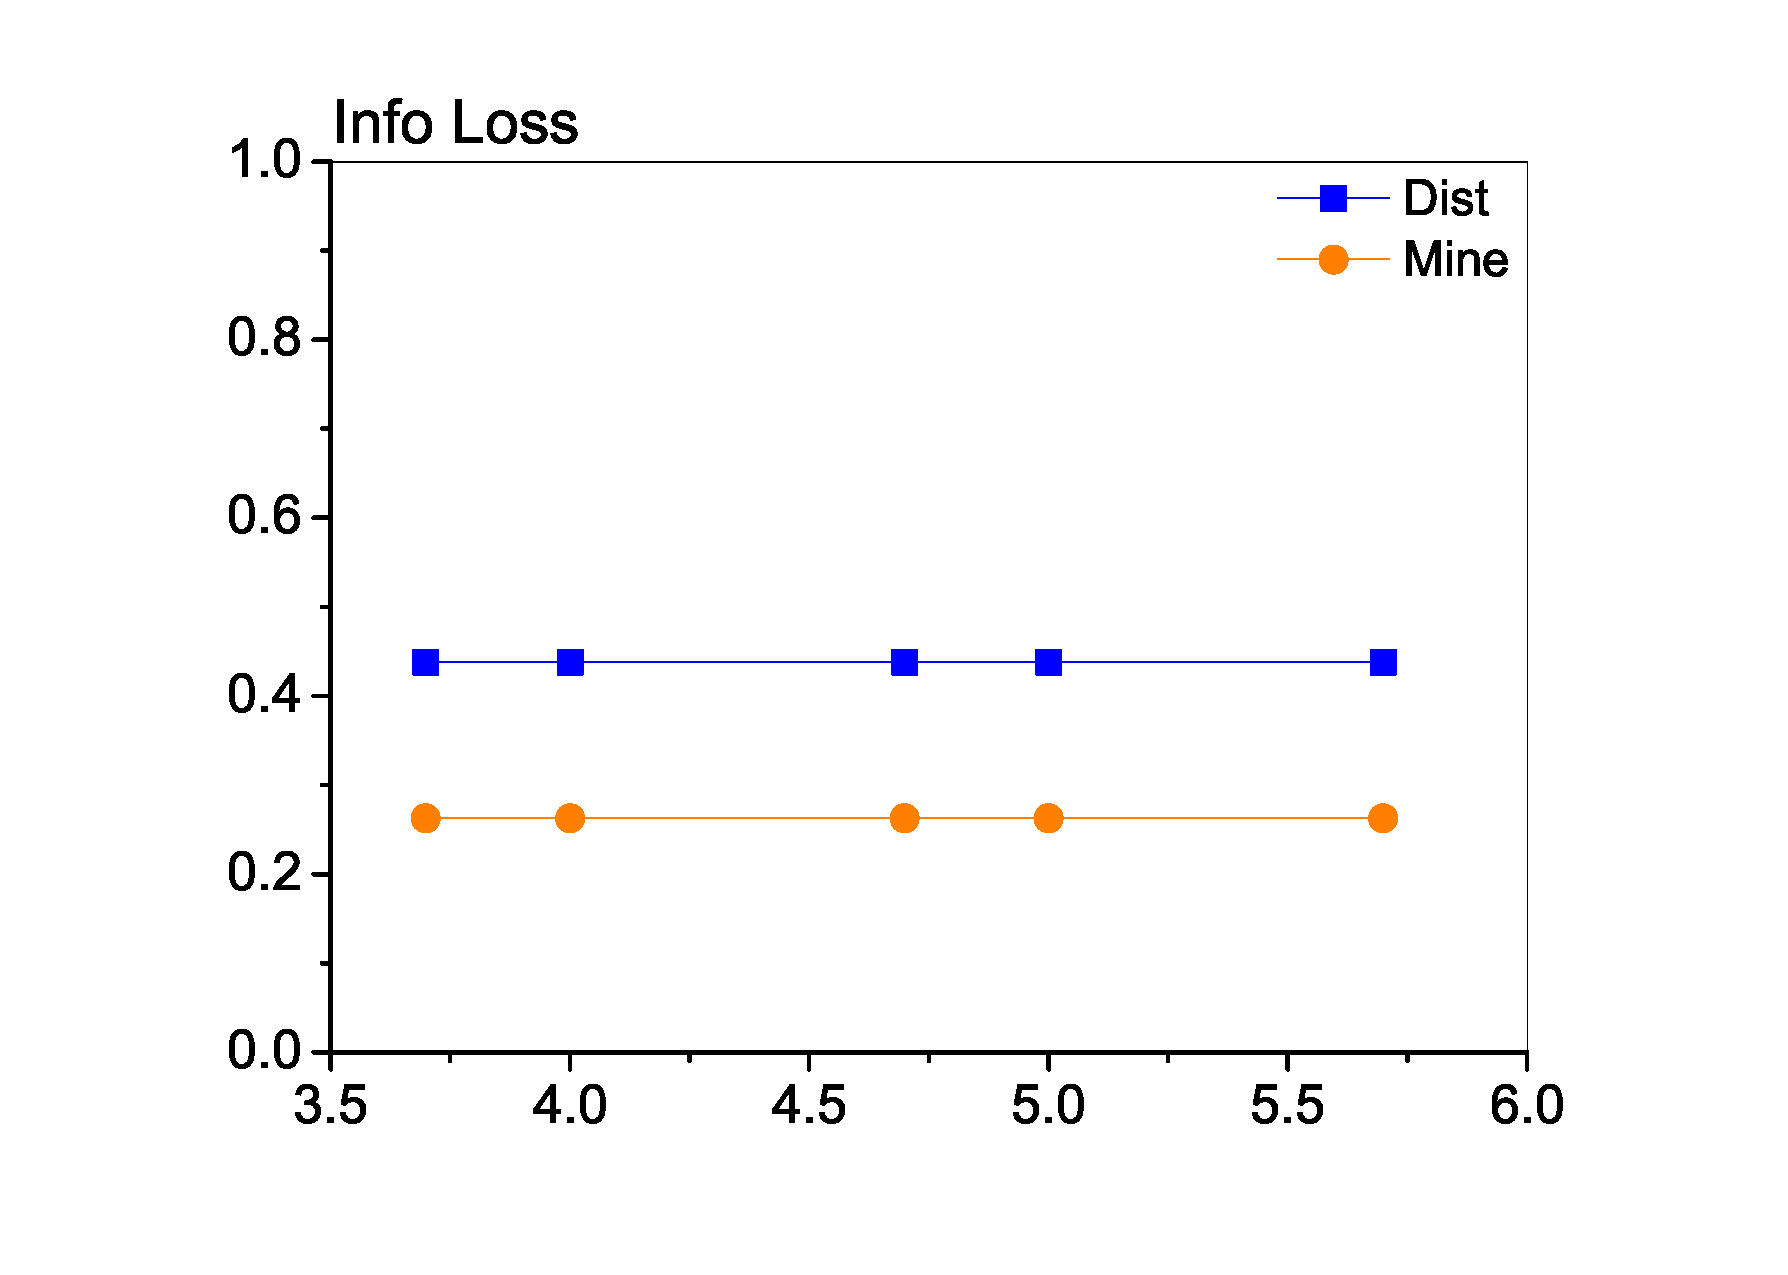
\includegraphics[width=5cm]{buffersizeavg.eps}
\end{minipage}%
}
\subfigure[Time Performance]{
\begin{minipage}[c]{0.4\textwidth}
\centering
  \includegraphics[width=5cm]{buffersize.eps}
\end{minipage}%
}
\caption{Variation of Buffer Size $b_{max}$ ($\rho=0.7$)}\label{fig:buffersize}
\end{figure}

Next experiment (See Figure \ref{fig:buffersize}) illustrates the impact of varying $b_{max}$ on performance.
We choose $WV$ as our target dataset since the number of
distinct \qids are relatively smaller than other datasets and our algorithm
can terminate even when we set a small $b_{max}$.

Note first that varying $b_{max}$ has no effect on the information loss which
indicates that this parameter is purely for performance tuning.
At lower values, increasing $b_{max}$ gives almost exponential
savings in running time. But as $b_{max}$ reaches a certain point, the speedup
saturates, which suggests that given the fixed size of the data,
when $B$ is large enough to accommodate all \qids at once after some iterations,
further increase in $b_{max}$ is not useful.
The line for $Mine$ hasn't saturdated because $Mine$ suppresses 
fewer items and retains more \qids, hence requires a much larger
buffer. 

\cut{%%%%%%%%%%%%%%%%% begin of cut %%%%%%%%%%%
\begin{figure}[tb]
\subfigure[Information Loss]{
\label{fig:rhoVar1}
\hspace{-4mm}
\begin{minipage}[c]{0.3\textwidth}
\centering
  \includegraphics[width=5cm]{rhoil.eps}
\end{minipage}%
}
\subfigure[Data Distribution]{
\label{fig:rhoVar2}
\begin{minipage}[c]{0.3\textwidth}
\centering
  \includegraphics[width=5cm]{rhoKL.eps}
\end{minipage}%
}
\subfigure[Rule Mining]{
\label{fig:rhoVar3}
\begin{minipage}[c]{0.3\textwidth}
\centering
  \includegraphics[width=5cm]{rhorule.eps}
\end{minipage}%
}
\caption{Variation of $\rho$ (from 0 to 1)}\label{fig:rho}
\end{figure}

\subsubsection{Variation of $\rho$}
In this section, we gives the performance of our algorithm with regard
to the variation of $\rho$. We take WV as our test data.
Figure \ref{fig:rhoVar1} shows that
the information loss decreases when $\rho$ becomes larger. The reason is
clear: as $\rho$ grows, there are fewer unsafe qids in the data and
fewer suppressions need to be executed and hense less information less.
Figure \ref{fig:rhoVar2} shows that data distribution
is better when $\rho$ becomes larger. The reason should also be attributed to
the fewer suppressions executed when $\rho$ becomes larger. Few suppressions mean
less disturbance to the original distribution.
Figure \ref{fig:rhoVar3} shows an interesting curve that ascends first,
reaches optimum at $\rho=0.5$,
then descends dramatically.
Small $\rho$ will lead to the fact that we may generate many rules in
the original dataset and the large information loss
causes the Jaccard similarity to be small. Since the partial suppression
may reduce the confidence of the rule, when $\rho$ becomes larger,
the Jaccard similarity also becomes small.
The sudden descending of the curve should be attributed to
the small number of rules left after heavy suppressions.
When $\rho$ is 0.9, we can not find any
association rule left in the dataset and we only find 1 rule in the
original dataset. Therefore, the value is 0.
}%%%%%%%%%%%% end of cut %%%%%%%%%%%%%%%

\subsection{A Comparison to Permutation Method}
In this section, we compare our algorithms with a permutation method
\cite{2011:TKDE:Anonymous}
which we call $M$.
The privacy model of $M$
states that the probability of associating any transaction $R \in T$ with
any sensitive item $e \in D_S(T)$ is below $1/p$, where $p$ is known as
a privacy degree. This model is similar to ours when $\rho = 1/p$,
which allows us to compare three variants of our algorithm against
$M$ where $p=4, 6, 8, 10$ on dataset $WV$ which was reported in
\cite{2011:TKDE:Anonymous}.
Figure \ref{fig:permutation1} shows the result on K-L divergence.
All variants of our algorithm outperform $M$ in
preserving the data distribution. 
Figure \ref{fig:permutation2} shows timing results.
Even though $M$ is faster, our algorithms
terminate within acceptable time.

\begin{figure}[tb]
\centering
\subfigure[K-L Divergence]{\label{fig:permutation1}
\hspace{-4mm}
\begin{minipage}[c]{0.4\columnwidth}
%\flushleft
  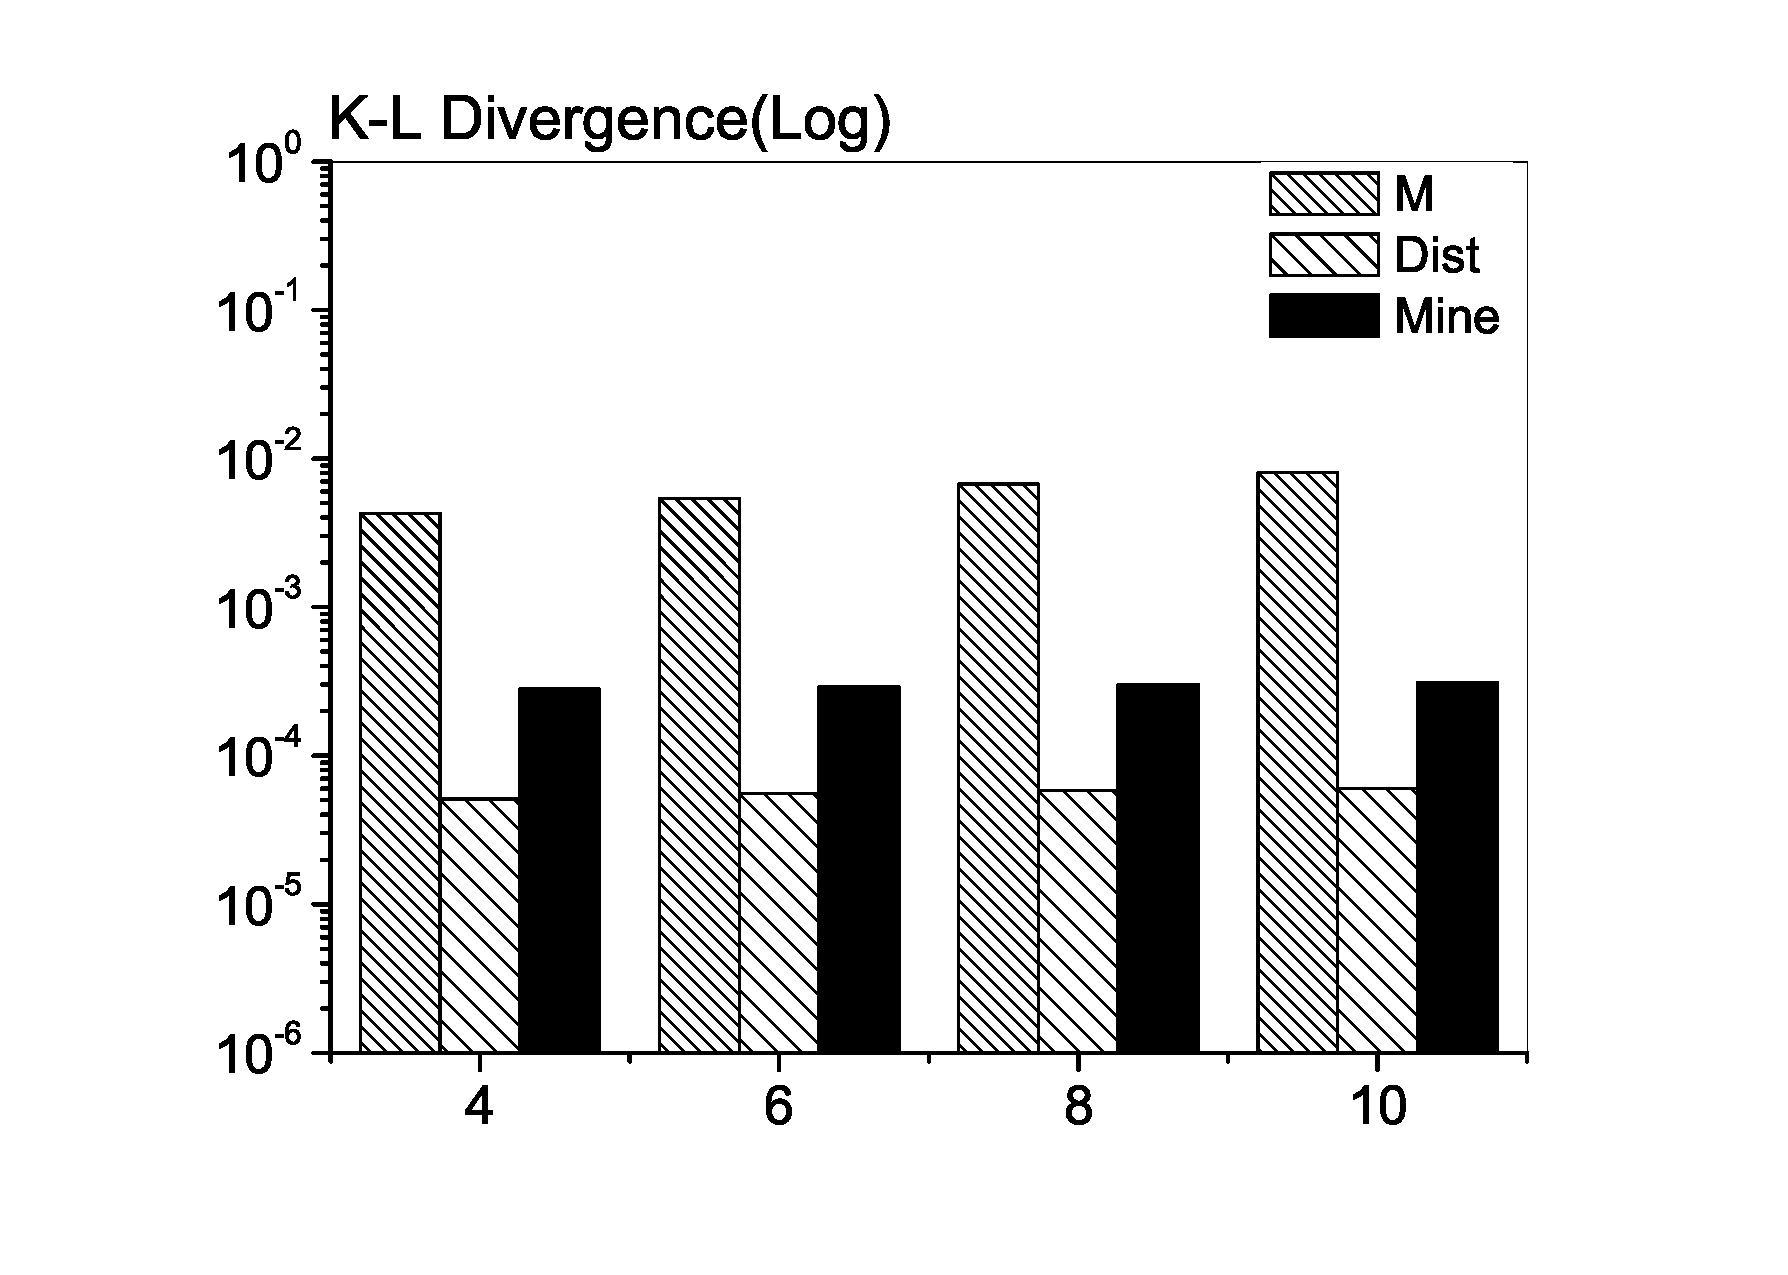
\includegraphics[width=5cm]{anatomy.eps}
\end{minipage}%
}
\subfigure[Time Performance]{\label{fig:permutation2}
\begin{minipage}[c]{0.4\columnwidth}
%\flushleft
  \includegraphics[width=5cm]{anatomytime.eps}
\end{minipage}%
}
\caption{Comparison with Permutation }
\end{figure}
